% Generated by Sphinx.
\def\sphinxdocclass{report}
\documentclass[letterpaper,10pt,french]{sphinxmanual}
\usepackage[utf8]{inputenc}
\DeclareUnicodeCharacter{00A0}{\nobreakspace}
\usepackage{cmap}
\usepackage[T1]{fontenc}
\usepackage{babel}
\usepackage{times}
\usepackage[Sonny]{fncychap}
\usepackage{longtable}
\usepackage{sphinx}
\usepackage{multirow}


\title{Documentation: dashboard professeur et développement dirigé par les tests}
\date{14 January 2015}
\release{0.1}
\author{Bryan Oberson}
\newcommand{\sphinxlogo}{}
\renewcommand{\releasename}{Version}
\makeindex

\makeatletter
\def\PYG@reset{\let\PYG@it=\relax \let\PYG@bf=\relax%
    \let\PYG@ul=\relax \let\PYG@tc=\relax%
    \let\PYG@bc=\relax \let\PYG@ff=\relax}
\def\PYG@tok#1{\csname PYG@tok@#1\endcsname}
\def\PYG@toks#1+{\ifx\relax#1\empty\else%
    \PYG@tok{#1}\expandafter\PYG@toks\fi}
\def\PYG@do#1{\PYG@bc{\PYG@tc{\PYG@ul{%
    \PYG@it{\PYG@bf{\PYG@ff{#1}}}}}}}
\def\PYG#1#2{\PYG@reset\PYG@toks#1+\relax+\PYG@do{#2}}

\expandafter\def\csname PYG@tok@gd\endcsname{\def\PYG@tc##1{\textcolor[rgb]{0.63,0.00,0.00}{##1}}}
\expandafter\def\csname PYG@tok@gu\endcsname{\let\PYG@bf=\textbf\def\PYG@tc##1{\textcolor[rgb]{0.50,0.00,0.50}{##1}}}
\expandafter\def\csname PYG@tok@gt\endcsname{\def\PYG@tc##1{\textcolor[rgb]{0.00,0.27,0.87}{##1}}}
\expandafter\def\csname PYG@tok@gs\endcsname{\let\PYG@bf=\textbf}
\expandafter\def\csname PYG@tok@gr\endcsname{\def\PYG@tc##1{\textcolor[rgb]{1.00,0.00,0.00}{##1}}}
\expandafter\def\csname PYG@tok@cm\endcsname{\let\PYG@it=\textit\def\PYG@tc##1{\textcolor[rgb]{0.25,0.50,0.56}{##1}}}
\expandafter\def\csname PYG@tok@vg\endcsname{\def\PYG@tc##1{\textcolor[rgb]{0.73,0.38,0.84}{##1}}}
\expandafter\def\csname PYG@tok@m\endcsname{\def\PYG@tc##1{\textcolor[rgb]{0.13,0.50,0.31}{##1}}}
\expandafter\def\csname PYG@tok@mh\endcsname{\def\PYG@tc##1{\textcolor[rgb]{0.13,0.50,0.31}{##1}}}
\expandafter\def\csname PYG@tok@cs\endcsname{\def\PYG@tc##1{\textcolor[rgb]{0.25,0.50,0.56}{##1}}\def\PYG@bc##1{\setlength{\fboxsep}{0pt}\colorbox[rgb]{1.00,0.94,0.94}{\strut ##1}}}
\expandafter\def\csname PYG@tok@ge\endcsname{\let\PYG@it=\textit}
\expandafter\def\csname PYG@tok@vc\endcsname{\def\PYG@tc##1{\textcolor[rgb]{0.73,0.38,0.84}{##1}}}
\expandafter\def\csname PYG@tok@il\endcsname{\def\PYG@tc##1{\textcolor[rgb]{0.13,0.50,0.31}{##1}}}
\expandafter\def\csname PYG@tok@go\endcsname{\def\PYG@tc##1{\textcolor[rgb]{0.20,0.20,0.20}{##1}}}
\expandafter\def\csname PYG@tok@cp\endcsname{\def\PYG@tc##1{\textcolor[rgb]{0.00,0.44,0.13}{##1}}}
\expandafter\def\csname PYG@tok@gi\endcsname{\def\PYG@tc##1{\textcolor[rgb]{0.00,0.63,0.00}{##1}}}
\expandafter\def\csname PYG@tok@gh\endcsname{\let\PYG@bf=\textbf\def\PYG@tc##1{\textcolor[rgb]{0.00,0.00,0.50}{##1}}}
\expandafter\def\csname PYG@tok@ni\endcsname{\let\PYG@bf=\textbf\def\PYG@tc##1{\textcolor[rgb]{0.84,0.33,0.22}{##1}}}
\expandafter\def\csname PYG@tok@nl\endcsname{\let\PYG@bf=\textbf\def\PYG@tc##1{\textcolor[rgb]{0.00,0.13,0.44}{##1}}}
\expandafter\def\csname PYG@tok@nn\endcsname{\let\PYG@bf=\textbf\def\PYG@tc##1{\textcolor[rgb]{0.05,0.52,0.71}{##1}}}
\expandafter\def\csname PYG@tok@no\endcsname{\def\PYG@tc##1{\textcolor[rgb]{0.38,0.68,0.84}{##1}}}
\expandafter\def\csname PYG@tok@na\endcsname{\def\PYG@tc##1{\textcolor[rgb]{0.25,0.44,0.63}{##1}}}
\expandafter\def\csname PYG@tok@nb\endcsname{\def\PYG@tc##1{\textcolor[rgb]{0.00,0.44,0.13}{##1}}}
\expandafter\def\csname PYG@tok@nc\endcsname{\let\PYG@bf=\textbf\def\PYG@tc##1{\textcolor[rgb]{0.05,0.52,0.71}{##1}}}
\expandafter\def\csname PYG@tok@nd\endcsname{\let\PYG@bf=\textbf\def\PYG@tc##1{\textcolor[rgb]{0.33,0.33,0.33}{##1}}}
\expandafter\def\csname PYG@tok@ne\endcsname{\def\PYG@tc##1{\textcolor[rgb]{0.00,0.44,0.13}{##1}}}
\expandafter\def\csname PYG@tok@nf\endcsname{\def\PYG@tc##1{\textcolor[rgb]{0.02,0.16,0.49}{##1}}}
\expandafter\def\csname PYG@tok@si\endcsname{\let\PYG@it=\textit\def\PYG@tc##1{\textcolor[rgb]{0.44,0.63,0.82}{##1}}}
\expandafter\def\csname PYG@tok@s2\endcsname{\def\PYG@tc##1{\textcolor[rgb]{0.25,0.44,0.63}{##1}}}
\expandafter\def\csname PYG@tok@vi\endcsname{\def\PYG@tc##1{\textcolor[rgb]{0.73,0.38,0.84}{##1}}}
\expandafter\def\csname PYG@tok@nt\endcsname{\let\PYG@bf=\textbf\def\PYG@tc##1{\textcolor[rgb]{0.02,0.16,0.45}{##1}}}
\expandafter\def\csname PYG@tok@nv\endcsname{\def\PYG@tc##1{\textcolor[rgb]{0.73,0.38,0.84}{##1}}}
\expandafter\def\csname PYG@tok@s1\endcsname{\def\PYG@tc##1{\textcolor[rgb]{0.25,0.44,0.63}{##1}}}
\expandafter\def\csname PYG@tok@gp\endcsname{\let\PYG@bf=\textbf\def\PYG@tc##1{\textcolor[rgb]{0.78,0.36,0.04}{##1}}}
\expandafter\def\csname PYG@tok@sh\endcsname{\def\PYG@tc##1{\textcolor[rgb]{0.25,0.44,0.63}{##1}}}
\expandafter\def\csname PYG@tok@ow\endcsname{\let\PYG@bf=\textbf\def\PYG@tc##1{\textcolor[rgb]{0.00,0.44,0.13}{##1}}}
\expandafter\def\csname PYG@tok@sx\endcsname{\def\PYG@tc##1{\textcolor[rgb]{0.78,0.36,0.04}{##1}}}
\expandafter\def\csname PYG@tok@bp\endcsname{\def\PYG@tc##1{\textcolor[rgb]{0.00,0.44,0.13}{##1}}}
\expandafter\def\csname PYG@tok@c1\endcsname{\let\PYG@it=\textit\def\PYG@tc##1{\textcolor[rgb]{0.25,0.50,0.56}{##1}}}
\expandafter\def\csname PYG@tok@kc\endcsname{\let\PYG@bf=\textbf\def\PYG@tc##1{\textcolor[rgb]{0.00,0.44,0.13}{##1}}}
\expandafter\def\csname PYG@tok@c\endcsname{\let\PYG@it=\textit\def\PYG@tc##1{\textcolor[rgb]{0.25,0.50,0.56}{##1}}}
\expandafter\def\csname PYG@tok@mf\endcsname{\def\PYG@tc##1{\textcolor[rgb]{0.13,0.50,0.31}{##1}}}
\expandafter\def\csname PYG@tok@err\endcsname{\def\PYG@bc##1{\setlength{\fboxsep}{0pt}\fcolorbox[rgb]{1.00,0.00,0.00}{1,1,1}{\strut ##1}}}
\expandafter\def\csname PYG@tok@kd\endcsname{\let\PYG@bf=\textbf\def\PYG@tc##1{\textcolor[rgb]{0.00,0.44,0.13}{##1}}}
\expandafter\def\csname PYG@tok@ss\endcsname{\def\PYG@tc##1{\textcolor[rgb]{0.32,0.47,0.09}{##1}}}
\expandafter\def\csname PYG@tok@sr\endcsname{\def\PYG@tc##1{\textcolor[rgb]{0.14,0.33,0.53}{##1}}}
\expandafter\def\csname PYG@tok@mo\endcsname{\def\PYG@tc##1{\textcolor[rgb]{0.13,0.50,0.31}{##1}}}
\expandafter\def\csname PYG@tok@mi\endcsname{\def\PYG@tc##1{\textcolor[rgb]{0.13,0.50,0.31}{##1}}}
\expandafter\def\csname PYG@tok@kn\endcsname{\let\PYG@bf=\textbf\def\PYG@tc##1{\textcolor[rgb]{0.00,0.44,0.13}{##1}}}
\expandafter\def\csname PYG@tok@o\endcsname{\def\PYG@tc##1{\textcolor[rgb]{0.40,0.40,0.40}{##1}}}
\expandafter\def\csname PYG@tok@kr\endcsname{\let\PYG@bf=\textbf\def\PYG@tc##1{\textcolor[rgb]{0.00,0.44,0.13}{##1}}}
\expandafter\def\csname PYG@tok@s\endcsname{\def\PYG@tc##1{\textcolor[rgb]{0.25,0.44,0.63}{##1}}}
\expandafter\def\csname PYG@tok@kp\endcsname{\def\PYG@tc##1{\textcolor[rgb]{0.00,0.44,0.13}{##1}}}
\expandafter\def\csname PYG@tok@w\endcsname{\def\PYG@tc##1{\textcolor[rgb]{0.73,0.73,0.73}{##1}}}
\expandafter\def\csname PYG@tok@kt\endcsname{\def\PYG@tc##1{\textcolor[rgb]{0.56,0.13,0.00}{##1}}}
\expandafter\def\csname PYG@tok@sc\endcsname{\def\PYG@tc##1{\textcolor[rgb]{0.25,0.44,0.63}{##1}}}
\expandafter\def\csname PYG@tok@sb\endcsname{\def\PYG@tc##1{\textcolor[rgb]{0.25,0.44,0.63}{##1}}}
\expandafter\def\csname PYG@tok@k\endcsname{\let\PYG@bf=\textbf\def\PYG@tc##1{\textcolor[rgb]{0.00,0.44,0.13}{##1}}}
\expandafter\def\csname PYG@tok@se\endcsname{\let\PYG@bf=\textbf\def\PYG@tc##1{\textcolor[rgb]{0.25,0.44,0.63}{##1}}}
\expandafter\def\csname PYG@tok@sd\endcsname{\let\PYG@it=\textit\def\PYG@tc##1{\textcolor[rgb]{0.25,0.44,0.63}{##1}}}

\def\PYGZbs{\char`\\}
\def\PYGZus{\char`\_}
\def\PYGZob{\char`\{}
\def\PYGZcb{\char`\}}
\def\PYGZca{\char`\^}
\def\PYGZam{\char`\&}
\def\PYGZlt{\char`\<}
\def\PYGZgt{\char`\>}
\def\PYGZsh{\char`\#}
\def\PYGZpc{\char`\%}
\def\PYGZdl{\char`\$}
\def\PYGZhy{\char`\-}
\def\PYGZsq{\char`\'}
\def\PYGZdq{\char`\"}
\def\PYGZti{\char`\~}
% for compatibility with earlier versions
\def\PYGZat{@}
\def\PYGZlb{[}
\def\PYGZrb{]}
\makeatother

\renewcommand\PYGZsq{\textquotesingle}

\begin{document}

\maketitle
\tableofcontents
\phantomsection\label{index::doc}
Table des matières:




\chapter{Introduction}
\label{introduction:introduction}\label{introduction:conception-du-dashboard-professeur-a-laide-du-developpement-dirige-par-les-tests}\label{introduction::doc}
Dans ce travail, je vais tout d'abord documenter mon travail pratique. Ce
travail consiste en la conception d'un dashboard pour les professeurs
utilisant le framework Django tout en essayant de programmer
avec le développement dirigé par les tests.
Ce dashboard fera partie d'un projet plus grand: un site d'e-learning pour les
mathématiques.
Tous les termes spécifiques tels que framework seront expliqués par la suite.

Cette documentation parlera tout d'abord de l'intérêt de ce travail pratique.
Il y aura aussi le wireframe du dashboard et un diagramme UML expliquant mes
différents modèles Django. J'expliquerai par la suite comment j'ai utilisé
les différentes technologies pour créer mon application et comment
je pourrai l'intégrer au projet final (le site) en essayant de souligner les
difficultés que je pourrai rencontrer pendant l'intégration.

Par la suite, j'essaierai de résumer les connaissances de bases relatives
au développement dirigé par les tests. Ceci consistera à expliquer les
différents termes et à surtout à expliquer comment cela fonctionne et quels
sont les avantages.

Finalement, j'expliquerai comment créer une ébauche de dashboard (créer un
dashboard complet étant trop long et trop compliqué à tester de par le nombre
important de boutons et de fonctionnalités) en utilisant ce fameux
développement dirigé par les tests


\chapter{Explications des termes spécifiques}
\label{introduction:explications-des-termes-specifiques}
Pour être sûr que tout le monde comprenne de quoi nous allons parler,
il va nous falloir expliquer le lexique spécifique à nos deux sujets:
dashboard professeur et développement dirigé par les tests.


\section{Framework}
\label{introduction:framework}
Un \textbf{framework}, ou \textbf{structure logicielle}, sert de base à un programme.
En effet, c'est de par ses structures de base que l'on peut le plus facilement
programmer. C'est donc une grande aide à tout informaticien. Les framework les
plus connus seraient, par exemple, Django, Bootstrap ou Ruby On Rails.

Il est important de noter que les frameworks sont souvent spécialisés dans un
langage informatique très précis. Par exemple, Django utilise Python, Bootstrap
utilise HTML et CSS et Ruby on Rails utilise Ruby.

Un framework est en autre très utile pour la programmation orientée objet. Ce
type de programmation permet d'établir des liens entre les différents objets.
Le framework aide à créer des classes et surtout des héritages.


\section{Classes et héritages}
\label{introduction:classes-et-heritages}
Les classes correspondent à un moule dans lequel on met différentes
informations pour créer un objet. Par exemple, pour une voiture, on pourrait
définir sa couleur, sa marque ou encore son age. Tout ce qu'il reste à faire
est de donner des valeurs à ces trois propriétés pour ``créer'' la voiture.

Le concept d'héritage n'est pas beaucoup plus compliqué. En effet, un héritage
consiste à créer une classe en prenant comme base les caractéristiques d'une
autre, ce qui nous permet d'en rajouter d'autre. Dans un cas qui nous
intéresserait plus, un élève possède comme spécificités un nom, un prénom et
une école. On peut grâce à ça créer une classe Professeur, qui aura les
mêmes caractéristiques mais à laquelle on pourrait ajouter la branche qu'il
enseigne.


\section{Diagramme UML}
\label{introduction:diagramme-uml}
Quand l'on possède de nombreuses classes, il devient indispensable de pouvoir
voir rapidement quelles relations ces classes entreprennent entre elles. Pour
ceci, le meilleur moyen de le faire est de créer un diagramme UML. Un diagramme
schématise les objets et indique leurs différentes relations (relation simple
avec une clé étrangère ou aussi plusieurs-à-plusieurs (ManyToMany)).

Il existe de nombreux programmes permettant de réaliser des diagrammes UML
clairs et présentables, comme boUML, argoUML ou Poseidon.


\section{Wireframe}
\label{introduction:wireframe}
Un \textbf{wireframe} est un schéma consistant à mettre en valeur les relations entre les
différentes pages d'un site web. Cela explique par exemple ce qu'il se passe si
l'on clique sur tel ou tel bouton. Cela consiste donc à pouvoir voir ou
exactement l'on peut aller en manipulant les fonctionnalités du site.


\chapter{Fonctionnalités du dashboard}
\label{dashboard:fonctionnalites-du-dashboard}\label{dashboard::doc}

\section{Accueil}
\label{dashboard:accueil}
Dans l'accueil, le professeur a la possibilité de voir les statistiques
hebdomadaires mais aussi de voir quelle classe a le mieux réussi ses exercices
au cours de la semaine. Cette page n'est pas la plus importante et sert simplement
de vue générale pour le professeur.


\section{Exercices}
\label{dashboard:exercices}
Dans l'onglet Exercices, le professeur pour tout d'abord voir très rapidement
l'état de ses différents exercices et chapitres, comme la date d'ajout,
le nombre de fois qu'il a été réalisé, et même voir selon les classes qui l'a
fait ou pas fait. Ceci est très utile si l'on veut suivre ses élèves assidument

Il pourra aussi y trouver des boutons qui lui permettront directement d'arriver
sur les formulaires de création d'exercices et de chapitres.


\section{Classes}
\label{dashboard:classes}
C'est dans l'onglet Classes que le professeur pourra réaliser le plus grand
nombre de tâches.

Tout d'abord, il lui sera possible de voir quels élèves appartiennent à cette
classe, mais aussi quel professeur(s) en est en charge, et leur date d'ajout.
Il pourra aussi ajouter des élèves et des professeurs mais aussi les supprimer.

Il pourra aussi voir quels devoirs ont été assignés à la classe, la date
d'assignation, le nombres de fois qu'il a été fait ou pas fait et finalement
le taux de réussite, c'est-à-dire combien de bonnes réponses ont été données par
rapport aux nombres de mauvaises réponses. Ceci peut être utile pour voir
si une classe à des problèmes avec tel ou tel exercice ou thème en général.


\section{Nouvelle classe}
\label{dashboard:nouvelle-classe}
C'est sur cette page qu'un professeur va pouvoir créer une nouvelle page. Pour
ceci, il lui suffira d'entrer le nom de la classe et de rajouter les élèves
en dessous. le bouton \textbf{+} permet de valider l'élève précédemment inscrit
et le rajouter dans une liste en dessous. Il ne reste qu'à valider la classe
qui se rajoutera dans le menu à gauche.


\section{Compte}
\label{dashboard:compte}
C'est depuis ce menu qu'il est possible d'atteindre son dashboard, mais aussi
de voir les informations relatives au compte. C'est aussi de par ce menu
déroulant qu'il peut se déconnecter.


\chapter{Documentation}
\label{documentation:documentation}\label{documentation::doc}

\section{Différentes technologies}
\label{documentation:differentes-technologies}
Pour créer mon application ( dashboard professeur ), j'ai fait recourt aux
technologies suivantes.


\subsection{HTML5 (Hypertext Markup Language)}
\label{documentation:html5-hypertext-markup-language}
HTML est la base de toute page web. En effet, c'est ce qui nous permet
d'afficher du texte, des images. Il est principalement utilisé avec CSS (pour la
mise en page) et JavaScript (pour l'interactivité des pages).

J'ai utilisé HTML5 pour faire le frontal ( plus connu sous le nom front-end ).
Le frontal correspond à ce que l'utilisateur voit. Il est opposé au back-end,
qui est la partie qui travaille derrière mais que l'utilisateur ne voit pas.


\subsection{CSS3 (Cascading Style Sheets)}
\label{documentation:css3-cascading-style-sheets}
CSS3 a été utilisé pour mettre en page mon code HTML. Cela a donc aussi
contribué à la partie front-end de mon application. C'est CSS qui permet de
modifier la police du texte, modifier la taille des images, ou encore
de modifier la couleur du font. CSS permet donc de rendre une page potable
pour l'oeil.


\subsection{Bootstrap}
\label{documentation:bootstrap}
Bootstrap est un framework qui contient du code HTML et CSS. J'ai utilisé
Bootstrap comme base pour mon dashboard en utilisant le modèle \emph{Charisma}
\footnote{
\href{http://usman.it/free-responsive-admin-template/}{http://usman.it/free-responsive-admin-template/}
}. L'avantage de Bootstrap est qu'il offre des
design adaptatifs, qui signifie que la mise en page va s'adapter à la taille de
l'écran.

Voici un exemple d'adaptation:

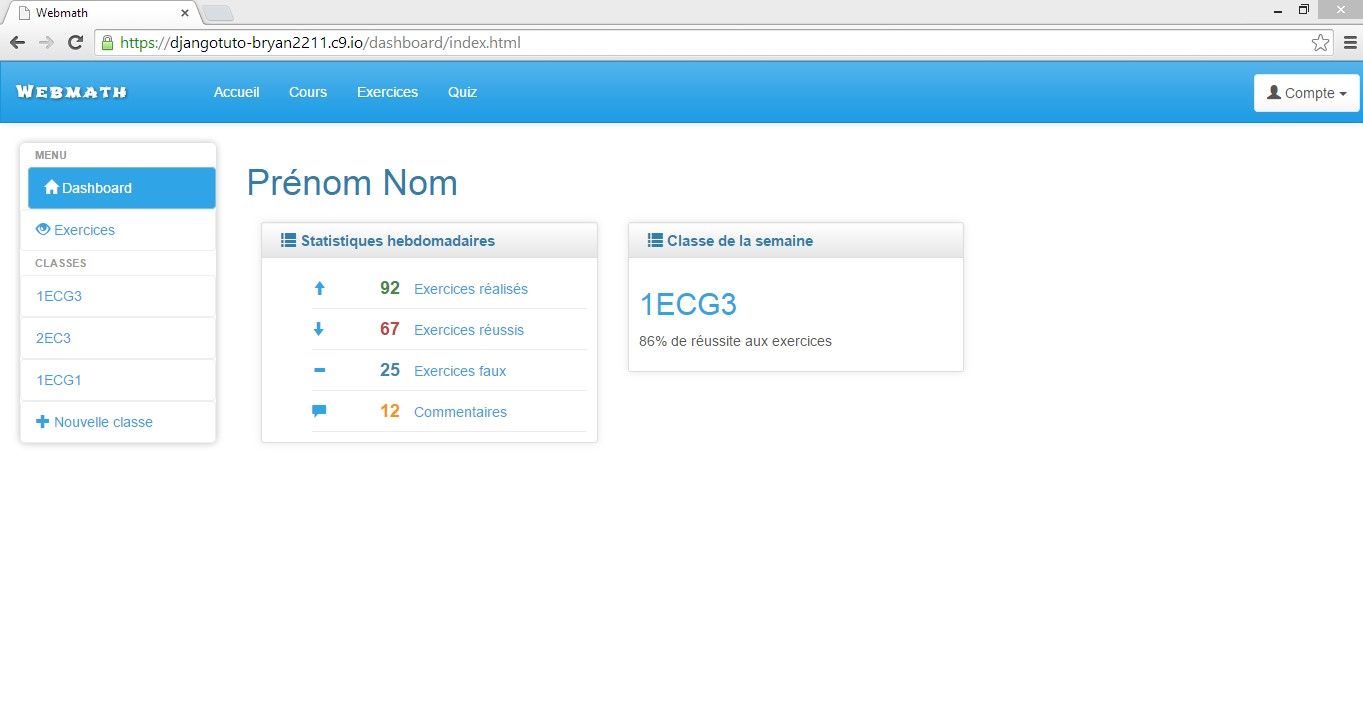
\includegraphics{source/images/fullscreen.png}

Voici à quoi ressemble le dashboard sur un écran d'ordinateur.

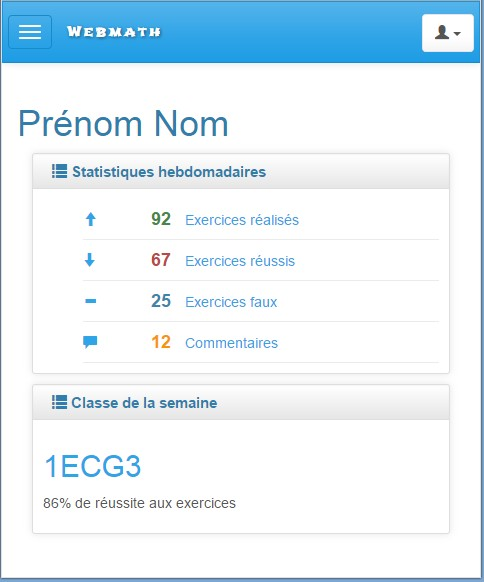
\includegraphics{source/images/smallscreen.png}

Et voici ce que la page devient si l'on zoome ou si l'on réduit la taille de la
fenêtre.


\subsection{Django}
\label{documentation:django}
Django est un framework spécialisé dans Python. C'est un des framework les plus
utilisés.


\section{Application au projet}
\label{documentation:application-au-projet}
Dans le projet final, qui, rappelons-le, consistera en un site d'e-learning pour
les mathématiques, ma partie pratique sera le dashboard professeur, donc
l'endroit ou les professeurs pourront gérer leurs exercices, leurs classes et
leurs élèves. La raison pour laquelle cette partie du site est si importante
est que sans un dashboard parfaitement opérationnel, il deviendrait chaotique
pour les professeurs de gérer leurs différentes responsabilités.

Toutes les fonctionnalités ayant déjà été expliquées auparavant, je ne vais pas
repasser dessus.


\section{Wireframes, ou ``scénarios du site''}
\label{documentation:wireframes-ou-scenarios-du-site}

\section{Modèles et diagrammes UML}
\label{documentation:modeles-et-diagrammes-uml}

\subsection{Modèles User}
\label{documentation:modeles-user}
Les modèles User, c'est-à-dire les modèles qui héritent du modèle Django de base
User, sont les plus importants dans la conception de mon dashboard. En effet, il
y a tout d'abord Student, dont les propriétés sont le nom, le prénom et le
niveau. Ce sont donc les caractéristiques de base d'un utilisateur qui doit
apprendre.

De ce modèle Student hérite une classe Teachers, qui est évidemment le point
central de notre travail. Etant donné qu'il hérite de Students, il possède
les mêmes propriétés qu'un élève. Je ne trouve pas nécessaire d'ajouter une
caractéristique, bien qu'on puisse par exemple ajouter la branche qu'il
enseigne, même si cela peut paraître superflu sur un site pour apprendre
les mathématiques.

Grâce à ces utilisateurs, nous pouvons créer des classes ou groupes, avec le
modèle Group. Celui-ci possède un nom, un ou plusieurs élèves ou professeurs et
des exercices assignés en devoir.


\subsection{Modèles d'exercices ou de cours}
\label{documentation:modeles-d-exercices-ou-de-cours}
M'occupant du professeur, je dois aussi pouvoir gérer les exercices, chapitres,
QCM ou cours qu'il voudra ajouter sur le site.

Partons tout d'abord du modèle Theme, qui possède la propriété name. Grâce à
cette caractéristique nous pouvons définir la classe Chapter. En effet, quand un
professeur crée un chapitre, il devrait pouvoir choisir un thème, mais aussi un
nom, ce qui explique l'entrée name.

A ces chapitres peuvent être associés des exercices, c'est pourquoi il y a le
modèle Exercise, où il est décrit les utilisateurs, le propriétaire, les
chapitres dans lequel il appartient, quand il a été écrit ou mis-à-jour,
son niveau, des indices et des commentaires. Ce modèle est le centre de toutes
les classes concernant les exercices.


\subsection{Diagramme UML}
\label{documentation:diagramme-uml}

\section{Implémentation avec le reste du projet}
\label{documentation:implementation-avec-le-reste-du-projet}\paragraph{Note de bas de page}


\chapter{Développement dirigé par les tests}
\label{tdd::doc}\label{tdd:developpement-dirige-par-les-tests}
Le développement dirigé par les tests, grossièrement traduit de l'anglais Test
Driven Development, est une technique de programmation utilisée par beaucoup de
programmeurs.

En effet, c'est grâce à cette technique que l'on peut le mieux s'assurer de la
fonctionnalité du site et de la simplicité du code. Dans un travail de longue
haleine, cette méthode devient nécessaire pour ne pas être redondant dans son
code et pour le rendre le plus clair possible.

Dans cette première partie, nous allons nous intéresser au côté théorique de ce
type de programmation avant de se lancer dans un réel projet.

Le développement dirigé par les tests est composé de deux tests importants et
bien différents.


\section{Le test fonctionnel}
\label{tdd:le-test-fonctionnel}
Le test fonctionnel, comme son nom l'indique, cherche à tester la fonctionnalité
du site. Plus précisément, il se met du côté de l'utilisateur du site. Il va par
exemple vérifier que les titres et les textes apparaissent, mais il va aussi
regarder si les différents boutons ou champs de textes marchent.

Voici un exemple de test fonctionnel:

\textbf{Mettre un test fonctionnel plus tard}

Nous pouvons déjà voir que les commentaires sont énormément présents dans ce
test. En effet, la convention est que l'on crée un scénario pour expliquer
exactement ce que l'on teste. Dans cet exemple, nous avons le professeur
Jean-Paul qui entend parler d'un site pour apprendre les mathématiques où il y a
un dashboard qui lui permet de gérer son travail. Il va donc essayer
tous les boutons et toutes les fonctionnalités.

Evidemment, cela peut paraître obsolète, mais ça vous aide à vous y retrouver.


\section{Le test unitaire}
\label{tdd:le-test-unitaire}
Le test unitaire, lui, se base plus sur le point de vue du programmateur. Si on
aurait pu considérer le test fonctionnel comme un test externe, le test unitaire
lui serait le test interne. Ce qu'il test ne sera jamais vu, car il permet de
vérifier que le code est le plus propre et le plus simple possible.

Voici un exemple:

\textbf{Test unitaire}


\section{Le cycle du développement dirigé par les tests}
\label{tdd:le-cycle-du-developpement-dirige-par-les-tests}
Quand on veut programmer à l'aide du développement dirigé par les tests, on
tente de suivre un certain cycle:
\begin{enumerate}
\item {} 
Tout d'abord, il est \textbf{impératif} d'écrire un test avant même d'écrire
n'importe quelle ligne de code. En effet, l'idée du Test Driven Development
est d'être sûr qu'un test échoue avant d'écrire notre code. Le test peut
être fonctionnel ou unitaire, cela dépendant de la partie de votre
application que vous souhaitez développer. Vous allez évidemment recevoir
un message disant que votre test a échoué, mais c'est normal étant
donné que vous n'avez rien codé. Cela consiste donc à essayer un
programme encore non-existant.

\item {} 
Ensuite seulement, le but est d'écrire un minimum de code possible
pour que le test précédemment lancé fonctionne. Il faut seulement s'occuper
de ce que le test cherchait à essayer, pas plus, pas moins.

\item {} 
Une fois que vous pensez avoir accompli ce que le test de la première étape
vous disait avoir raté, vous pouvez relancer ce test. Si le résultat
est positif, vous pouvez passer à l'étape suivante. Dans le cas contraire,
il va vous falloir refaire l'étape 2 et 3 jusqu'à ce que le test soit
positif.

\item {} 
L'étape finale: il va falloir réécrire et réstructurer le code précédent
histoire qu'il soit plus agréable à l'oeil et le rendre plus lisible.
Il faut faire très attention durant cette étape à ne rien rajouter ou
enlever. Le code doit garder le même résultat.

\end{enumerate}

Une fois que ces 4 étapes ont été effectuées, il ne reste évidemment qu'à
recommencer avec une autre fonctionnalité de l'application, jusqu'à
que celle-ci soit finie.


\section{Gain de temps?}
\label{tdd:gain-de-temps}
En lisant ces 4 étapes répétitives, on ne peut que se demander si le Test
Driven Development et son cycle compliqué est réellement un atout et un gain
de temps pour le programmeur.

Il est clair que, sur un travail de petite taille, tout coder n'aurait pas
énormément de sens, car tout peut être facilement essayable par soi-même.
Dans le cas d'un travail d'une certaine consistance, ce n'est pas pareil.
C'est uniquement en testant que l'on peut être sûr de son code, car cela
signifie que notre code est valide, et devrait le rester.


\chapter{Débuter un projet}
\label{projet1:debuter-un-projet}\label{projet1::doc}
Pour comprendre grâce à la pratique, nous allons au cours de ce travail établir un dashboard permettant à un
professeur de gérer des classes et des exercices sur un site d'e-learning pour les mathématiques grâce à Django, un framework fonctionnant avec Python.


\section{Eléments requis}
\label{projet1:elements-requis}
Pour pouvoir parfaitement suivre ce guide, il nous faudra les éléments suivants afin de réaliser les tests:
\begin{itemize}
\item {} 
\textbf{Django 1.7:} en effet, il va vous falloir django, car c'est le framework que l'on va utiliser. Pour le télécharger,
il suffit de taper la commande suivante avec pip:

\begin{Verbatim}[commandchars=\\\{\}]
sudo pip3 install django==1.7
\end{Verbatim}

Si vous utilisez Windows, vous pouvez enlever \emph{sudo}.

\item {} 
\textbf{Selenium:} Selenium est un outil permettant de gérer les navigateurs avec des commandes. Ceci nous sera utile pour les
tests fonctionnels (ce terme sera expliqué plus tard). Encore une fois, il est possible de le télécharger grâce à pip:

\begin{Verbatim}[commandchars=\\\{\}]
sudo pip3 install \PYGZhy{}\PYGZhy{}upgrade selenium
\end{Verbatim}

Encore une fois, le \emph{sudo} n'est pas nécessaire sur Windows.

Note: il est important de toujours utiliser la dernière version de Selenium. En effet, une version dépassée peut facilement se comporter de
façon non désirée. \footnote{
Inspiré de Test Driven Development With Python de Harry J.W. Percival
}

\end{itemize}

Une fois les éléments nécessaires installés, vous pouvez passer à la suite.


\section{Premier test}
\label{projet1:premier-test}
Le principe de base du Test Driven Development est d'écrire un test avant même de coder ce que le test doit vérifier. Pour notre exemple,
on devrait vérifier qu'il y ait le plus basique des éléments sur notre site: Django. On va donc créer un test fonctionnel pour voir s'il y a bien
le titre de Django sur la page d'accueil. Le test fonctionnel permet de nous assurer que notre site fonctionne et possède
la fonctionnalité la plus optimale qu'il soit.

Commençons donc par écrire ce code:

\begin{Verbatim}[commandchars=\\\{\},numbers=left,firstnumber=1,stepnumber=1]
\PYG{k+kn}{from} \PYG{n+nn}{selenium} \PYG{k+kn}{import} \PYG{n}{webdriver}

\PYG{n}{browser} \PYG{o}{=} \PYG{n}{webdriver}\PYG{o}{.}\PYG{n}{Firefox}\PYG{p}{(}\PYG{p}{)}
\PYG{n}{browser}\PYG{o}{.}\PYG{n}{get}\PYG{p}{(}\PYG{l+s}{\PYGZdq{}}\PYG{l+s}{http://localhost:8000}\PYG{l+s}{\PYGZdq{}}\PYG{p}{)}

\PYG{k}{assert} \PYG{l+s}{\PYGZdq{}}\PYG{l+s}{Django}\PYG{l+s}{\PYGZdq{}} \PYG{o+ow}{in} \PYG{n}{browser}\PYG{o}{.}\PYG{n}{title}

\PYG{n}{browser}\PYG{o}{.}\PYG{n}{quit}\PYG{p}{(}\PYG{p}{)}
\end{Verbatim}

Regardons une par une les lignes qui pourrait poser des problèmes de compréhensions:
\begin{enumerate}
\item {} 
Nous permet d'importer webdriver qui nous sera utile pour gérer les navigateurs web (dans ce cas, Firefox), nous permettant de les ouvrir,
d'aller à une URL ou de les fermer.

\end{enumerate}
\begin{enumerate}
\setcounter{enumi}{5}
\item {} 
Va basiquement nous dire si la page que l'on vient de charger (\href{http://localhost:8000}{http://localhost:8000}) contient le mot ``Django'' dans le titre.

\end{enumerate}

Comme on peut s'y attendre, du moins si on se rappelle du but d'un test, le test ne marchera pas. En effet, comme dit précédemment,
les tests sont faits pour évaluer quelque chose que l'on n'a pas encore fait, et pour nous aider à les faire le plus simplement possible.

\textbf{Quand on test, il ne faut pas avoir les tests qui échouent comme quelque chose de mal. Dans certains cas ( comme celui-ci),
ces tests sont attendus et recevoir un} \emph{False} \textbf{à la fin est donc un bon signe: notre test marche!}
\paragraph{Note de bas de page}



\renewcommand{\indexname}{Index}
\printindex
\end{document}
